\chapter{Validating our methodology}\label{sec:exps1}

In this chapter, we validate our methodology to evaluate the interpretability.
In particular we verify that our methodology that relies on policy unfolding can retrieve conclusions from user studies, e.g. we want that our measures of interpretability to change with parameter number inside a given policy class.

Because in this part of the manuscript we do evaluate learning capabilities of interpretable machine learning algorithms but solely their outputs, we use indirect imitation learning (cf. section~\ref{sec:imit}) to obtain policies from different classes.
Imitation learning is a great baseline to obtain policies from different classes.
Indeed, as long as there exists a supervised learning algorithm for a given model class, this algorithm can be used in e.g. algorithms~\ref{alg:dagger} or~\ref{alg:viper} to distillate the behaviour of any expert policy into the desired policy class. 
Furthermore, if policies are already available for some MDPs, we can simply re-use them as experts in e.g. algorithms~\ref{alg:dagger} or~\ref{alg:viper}.

\section{Obtaining policies from different classes}

\subsection{Policy classes}
\begin{table}[ht]
\centering
\small
\begin{tabular}{lll}
\hline
\textbf{Policy Class} & \textbf{Parameters} & \textbf{Training algorithm} \\
\hline
Linear Policies & Determined by state-action dimensions & Linear/Logistic Regression \\
Decision Trees & \{4, 8, 16, 64, 128\} nodes & CART \\
Oblique Decision Trees & \{4, 8, 16, 64, 128\} nodes & CART \\
relu neural networks & \{(2 ,2), (4, 4), (8, 8), (16, 16)\} weigths & SGD \\
\hline
\end{tabular}
\caption{Summary of policy classes parameters and supervised learning algorithms to fit experts.}
\label{tab:policy-classes}
\end{table}

We consider four policy classes for our baselines.
We consider linear policies that have been shown to be able to solve MuJoCo tasks~\cite{empirical-evidence}.
We fit linear policies to expert policies using simple linear (logistic) regressions with scikit-learn~\cite{scikit-learn} default implementation.
We also consider decision trees~\cite{breiman1984classification} and oblique decision trees~\cite{murthy1994system}.
Oblique decision trees are decision trees which does not necessarily partitions the input domain parallel to axes.
A test node in an oblique decision tree can be the linear combinations of two state features.
We give an example of an oblique decision tree unfolded for the Pong game in figure~\ref{lst:pong}.
\begin{figure}
  \centering
  \begin{minipage}{0.47\textwidth}
  \begin{lstlisting}[language=Python,style=mystyle]
  def play(x):
    if (x[12] - x[15]) <= 8.5:
        if (x[2] - x[7]) <= 139.5:
            if (x[12] - x[13]) <= 5.5:
                if (x[2] - x[7]) <= 130.5:
                    if (x[3] - x[14]) <= 110.5:
                        if (x[5] - x[11]) <= 13.5:
                            return 5
                        else:
                            return 4
                    else:
                        return 5
                else:
                    if (x[3] - x[11]) <= 173.5:
                        return 4
                    else:
                        return 1
            else:
                if (x[1] - x[2]) <= -80.5:
                    if (x[1] - x[3]) <= -28.5:
                        return 5
                    else:
                        return 3
                else:
                    if (x[3] - x[9]) <= 73.5:
                        return 2
                    else:
                        if (x[2] - x[17]) <= 100.5:
                            return 2
                        else:
                            return 4
        else:
            return 4
    else:
        if (x[1] - x[13]) <= 156.5:
            if (x[3] - x[12]) <= 143.0:
                if (x[1] - x[14]) <= 114.5:
                    return 4
                else:
                    return 1
            else:
                if (x[2] - x[11]) <= 150.5:
                    return 0
                else:
                    return 1
        else:
            return 4
  \end{lstlisting}
  \caption{Unfolded oblique decision tree policy with 11 nodes for Pong (RL objective value, i.e. episodic rewards of 16).}\label{lst:pong}
  \end{minipage}
  \hfill
  \begin{minipage}{0.47\textwidth}
  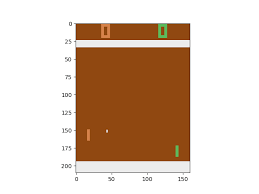
\includegraphics[width=1\textwidth]{images/images_part3/pong.png}
  \caption{The Pong game on Atari 2600.}\label{lst:generic-linear}
  \end{minipage}
  \end{figure}
We train trees using the default CART (algorithm~\ref{alg:cart} ~\cite{breiman1984classification}) implementation of scikit-learn with varying numbers of parameters (number of nodes in the tree).
We explain in more details how we adapt CART to return oblique decision trees in appendix~\ref{chap-app-imit}.
We also consider neural networks with relu activations~\cite{relunet} with varying number of parameters (total number of weights).

In Table~\ref{tab:policy-classes} we summarize the different policy classes we will consider for our study.
There is one class of linear policies, five classes of decision trees and oblique decision trees, each defined by the maximum number of nodes in the tree, and four classes or relu networks each defined by the number and sizes of hidden layers.

\subsection{Which expert policies to imitate with what algorithm?}
We do not have to re-run deep reinforcement learning algorithms \cite{dqn,ppo,deep-rl-relu1}, we can simply use the pre-trained policies from the stables-baselines3 zoo \cite{zoo} and try our methodology to evaluate their interpretability.
Depending on the MDPs, also called environments, we choose neural network policies trained with different deep reinforcement learning algorithms.
It is important to note that not all experts are compatible with all the variants of imitation learning algorithms.
Indeed, SAC experts \cite{deep-rl-relu1} are not compatible with VIPER~\cite{viper} because the latter only works for discrete actions.
We do not use PPO experts with VIPER either: despite working with discrete actions PPO do not compute a $Q$-function necessary for the samples re-weighting in VIPER.
All experts are compatible with Dagger~\cite{dagger}.
We also consider an additional imitation learning algorithm: behaviour cloning (BC)~\cite{behavior-cloning}.
BC is essentially just one iteration of Dagger imitation i.e. samples are only collected with the expert policy once before fitting a new poicy class.
For Dagger and VIPER we use 10 iterations of samples collections with experts and teacher policy (cf. algorithms~\ref{alg:dagger} and~\ref{alg:viper}) with different total samples budget.
In Table~\ref{tab:repet-distill}, we summarize the different algorithms used to imitate each expert.
We also specify the total number of samples collected during the imitations as well as the number of times we repet the imitations for statistical significance.

\begin{table}
  \centering
  \footnotesize
  \begin{tabular}{c|cccccc}
  \toprule
  Envs & BC & BC & Dagger & Dagger & VIPER & VIPER\\
   & 50K & 100K & 50K & 100K & 50K & 100K\\
  \midrule
  Classic& 50 (PPO, DQN)& 50 (PPO, DQN)& 50 (PPO, DQN)& 50 (PPO, DQN)&  50 (DQN) & 50 (DQN)\\
  OCAtari& 0 & 0 & 0 & 5 (DQN)&  0 & 5 (DQN)\\
  Mujoco& 10 (SAC)& 10 (SAC)& 10 (SAC)& 10 (SAC)&  0 & 0\\
  \bottomrule
  \end{tabular}
  \caption{Repetitions of each imitation learning algorithm on each environment. We specify from which deep RL algorithms expert policies from the zoo~\cite{zoo} come from in parentheses.}
  \label{tab:repet-distill}
\end{table}

\subsection{Which environments to consider?}
We evaluate the interpretability of policies for common environments in reinforcement learning research.
We consider the classic control tasks from gymnasium \cite{gymnasium}, MuJoCo robots from \cite{mujoco}, and Atari games from \cite{atari}.
For Atari games, since the state space is frame pixels that can't be interpreted, we use the object-centric version of the games from \cite{ocatari} in which states are objects in the frame and their positions.

In Table~\ref{tab:envs}, we summarize which environment we consider with their state-action space sizes and a threshold representing the rewards of a ``good'' policy.
In total, we compute across policy classes, imitation algorithms, experts origins, and environments, roughly 40 000 unique policies.

Using those 40 000 policies as baselines, we describe next the experimental setup used to evaluate their interpretability using our methodology.
All the experiments presented next run on a dedicated cluster of Intel Xeon Gold 6130 (Skylake-SP), 2.10GHz, 2 CPUs/node, 16 cores/CPU with a timeout of 4 hours per experiment.

\begin{table}[ht]
  \centering
  \small
  \begin{tabular}{lll}
  \hline
  \textbf{Classic} & \textbf{MuJoCo} & \textbf{OCAtari}\\
  \hline
  CartPole (4, 2, \textbf{490}) & Swimmer (8, 2, \textbf{300}) & Breakout (452, 4, \textbf{30})\\
  LunarLander (8, 4, \textbf{200}) & Walker2d (17, 6, \textbf{2000}) & Pong (20, 6, \textbf{14})\\
  //    Continuous (8, 2, \textbf{200}) & HalfCheetah (17, 6, \textbf{3000}) & SpaceInvaders (188, 6, \textbf{680})\\
  BipedalWalker (24, 4, \textbf{250}) & Hopper (11, 3, \textbf{2000}) & Seaquest (180, 18, \textbf{2000})\\
  MountainCar (2, 3, \textbf{90}) & \\
  //    Continuous (2, 1, \textbf{-110}) & \\
  Acrobot (6, 3, \textbf{-100}) & \\
  Pendulum (3, 1, \textbf{-400}) & \\
  \hline
  \end{tabular}
  \caption{Summary of considered environments (dimensions of states and number or dimensions of actions, \textbf{reward thresholds}). The rewards thresholds are obtained from gymnasium \cite{gymnasium}. For OCAtari environments, we choose the thresholds as the minimum between the DQN expert from \cite{zoo} and the human scores. We also adapt subjectively some thresholds that we find too restrictive especially for MuJoCo (for example, the PPO expert from \cite{zoo} has 2200 reward on Hopper while the default threshold was 3800).}
  \label{tab:envs}
  \end{table}


\section{Running the imitation learning algorithms}
Using the reinforcement learning evaluation library rliable~\cite{rliable}, we plot on figure \ref{fig:performance_comparison} the interquartile means (IQM, an estimator of the mean robust to outliers) of the baseline policies cumulative rewards averaged over 100 episodes.
For each imitation algorithm variant, we aggregate cumulative rewards over environments and policy classes.
We normalize the baselines cumulative rewards between expert and random agent cumulative rewards.

\begin{figure}[ht]
\centering
\begin{subfigure}{.33\textwidth}
  \centering
  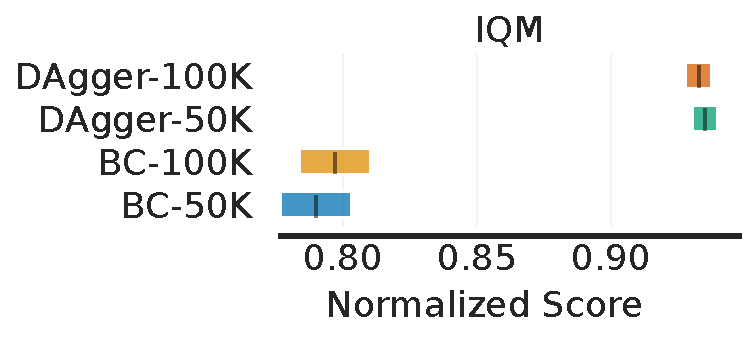
\includegraphics[width=\linewidth]{images/images_part3/ppo_expert_classic_control.pdf}
  \caption{Classic control, PPO expert}
  \label{fig:ppo_classic}
\end{subfigure}%
\begin{subfigure}{.33\textwidth}
  \centering
  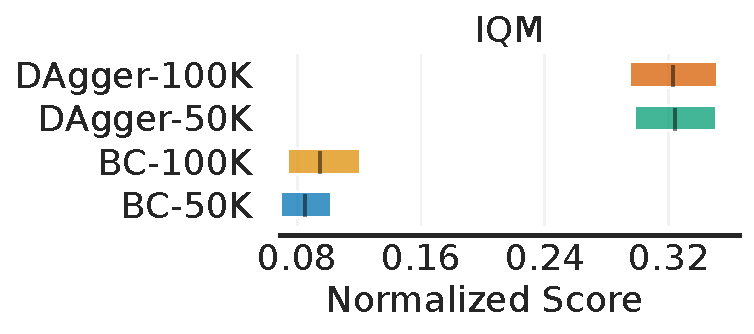
\includegraphics[width=\linewidth]{images/images_part3/sac_expert_mujoco.pdf}
  \caption{MuJoCo, SAC expert}
  \label{fig:sac_mujoco}
\end{subfigure}
\begin{subfigure}{.33\textwidth}
  \centering
  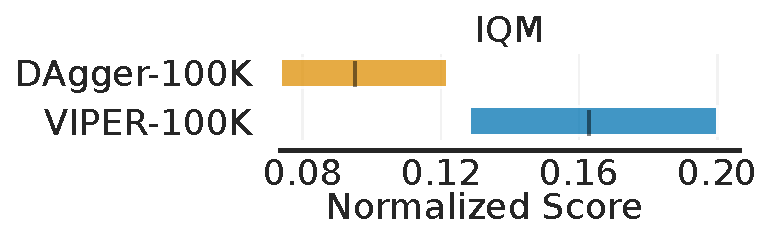
\includegraphics[width=\linewidth]{images/images_part3/dqn_expert_atari.pdf}
  \caption{OCAtari, DQN expert}
  \label{fig:dqn_atari}
\end{subfigure}%
\caption{Performance of different imitation learning algorithms on different environments. We plot the 95\% stratified bootstrapped confidence intervals around the IQMs.}
\label{fig:performance_comparison}
\end{figure}

\subsection{What is the best imitation algorithm?}

The key observation is that for tested environments (figures \ref{fig:ppo_classic},\ref{fig:sac_mujoco}), behavior cloning is not an efficient way to train baseline policies compared to Dagger.
This is probably because BC trains a policy to match the expert's actions on states visited by the expert, while Dagger trains a policy to take the expert's actions on the states visited by the trained policy~\cite{dagger}.
An other observation is that the best performing imitation algorithms for MuJoCo (Dagger, figure \ref{fig:sac_mujoco}) and OCAtari (VIPER, figure \ref{fig:dqn_atari}) obtain baselines that in average cannot match well the performances of the experts.
However baseline policies almost always match the experts on simple tasks like classic control (figure \ref{fig:ppo_classic}).

\subsection{What is the best policy class in terms of reward?}

\begin{figure}[ht]
    \centering
    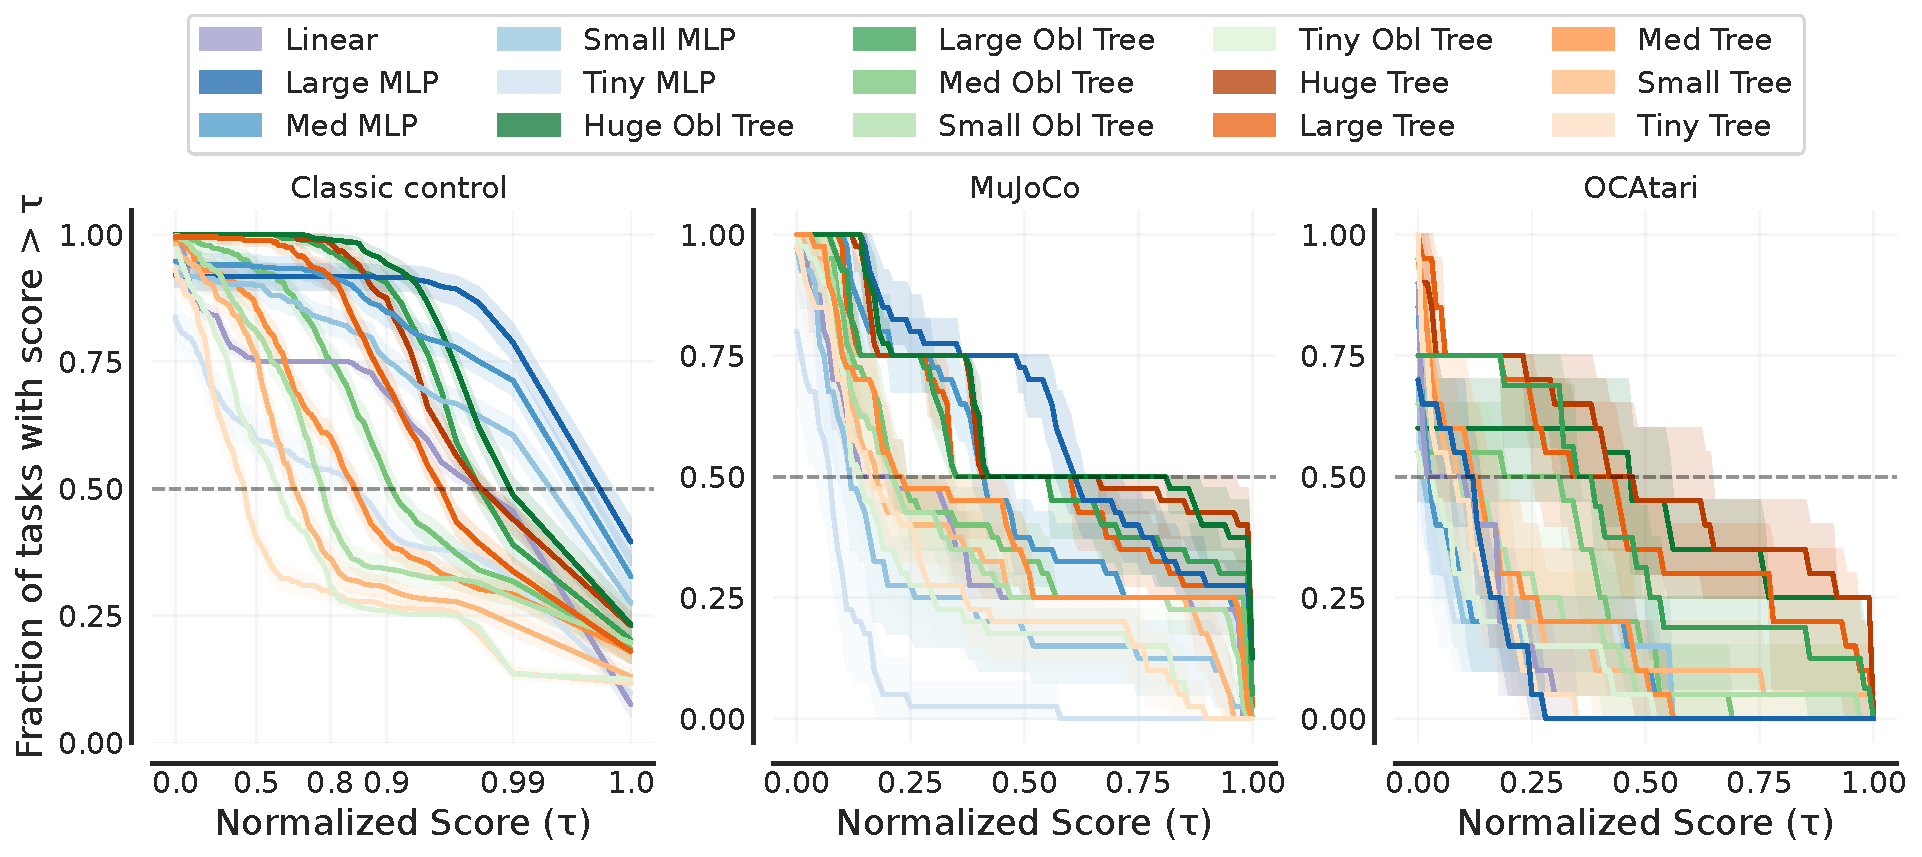
\includegraphics[trim={0 0 0 0.2cm},clip,width=0.9\linewidth]{images/images_part3/perf_profile_combined_100k.pdf}
    \caption{Performance profiles of different policy classes on different environments.}
    \label{fig:perf-combined}
\end{figure}

We also wonder if there is a policy class that matches expert performances more often than others across environments.
For that we plot performance profiles of the different policy classes obtained with a fixed expert and fixed imitation learning algorithm.
In particular, for each environments group we use the baseline policies obtained from the best performing imitation learning algorithm from figure \ref{fig:performance_comparison}.
From figure \ref{fig:perf-combined} we see that on classic control environments, neural networks tend to perform better than other classes while on OCAtari games, trees tend to perform better than other classes.
Now we move on to the interpretability evaluation.

\section{Is our methodology sound with respect to user studies?}

\begin{figure}
    \centering
    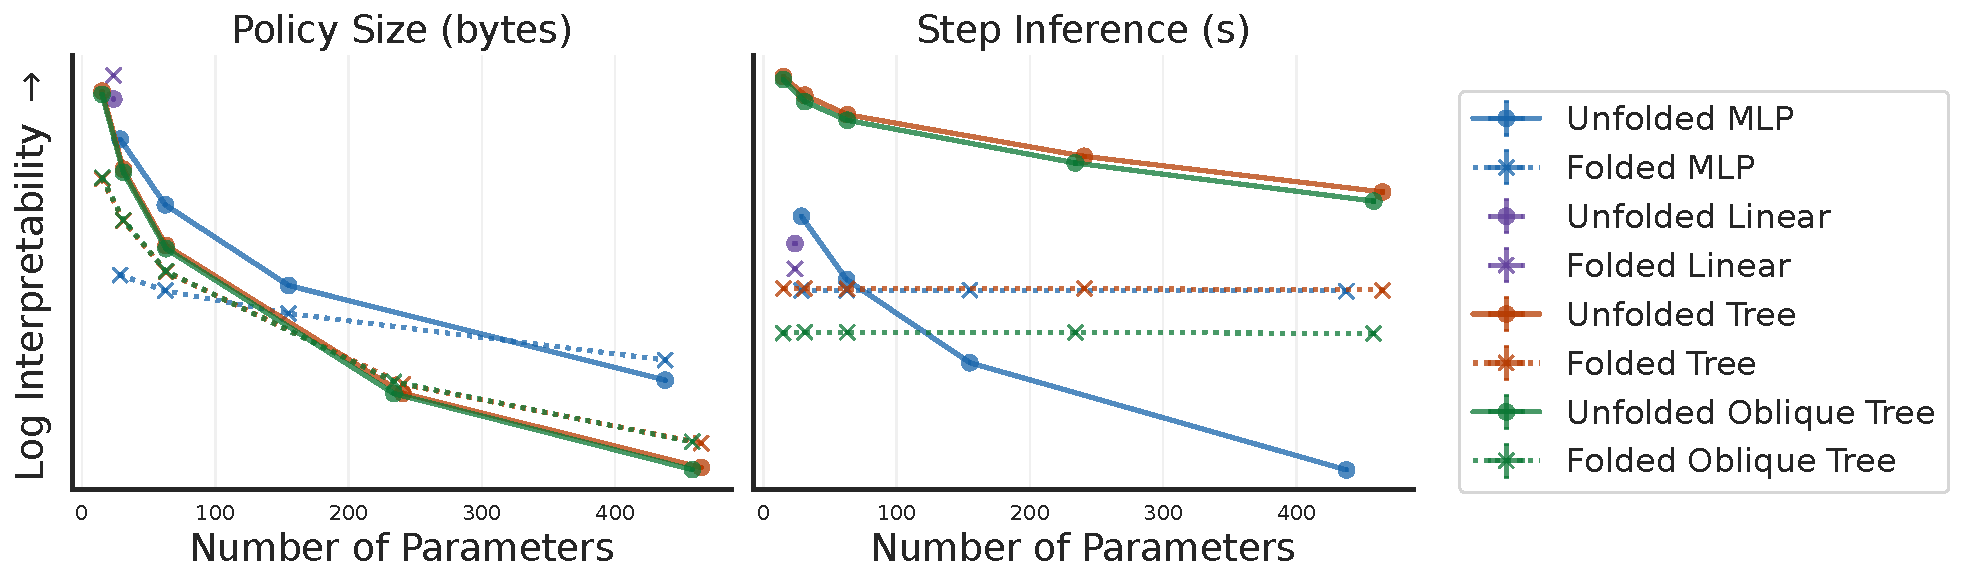
\includegraphics[width=1\linewidth]{images/images_part3/tree_sizes_memory_ppo_ci_ablation.pdf}
    \caption{Policies interpretability on classic control environments. We plot 95\% stratified bootstrapped confidence intervals around means in both axes. In each sub-plot, interpreatbility is measured with either bytes or inference speed.}
    \label{fig:abl-proxies}
\end{figure}

In this section, we compute the step inference times, as well as the policy size for both the folded and unfolded variant of each policy (cf. section~\ref{sec:unfold}) obtained for classic control environments with Dagger-100K.
To unfold policies, we convert them into Python programs formatted with PEP 8 (comparing other unfolding formats such as ONNX \url{https://github.com/onnx/onnx} is left to future work).
We ensure that all policies operations are performed sequentially, similarly to how a humand would operate, and compute the metrics for each policy on 100 episodes using the same CPUs.

\subsection{Is it necessary to unfold policies to compute interpretability metrics?}
We see on figure \ref{fig:abl-proxies} that folded policies of the same class almost always give similar interpretability values (dotted lines) despite having very different number of parameters.
Hence, measuring folded policies interpretability would contradict established results from user studies such as, e.g., trees of different sizes have different levels of interpretability~\cite{study-4}. 

\subsection{Is there a best policy class in terms of interpretability?}
User studies from~\cite{study-1,study-2,study-3} show that decision trees are easier to understand than models involving mathematical equations like oblique trees, linear maps, and neural networks.
However,~\cite{lipton} states that for a human wanting to have a global idea of the inference of a policy, a compact neural network can be more interpretable than a very deep decision tree.
In figure \ref{fig:abl-proxies}, we show that inference speed and memory size of unfolded policies help us capture those nuances: policy interpretability does not only depend on the policy class but also on the metric choice.
Indeed, when we measure interpretability with inference times, we do observe that trees are more interpretable than neural networks.
However, when measuring interpretability with policy size, we observe that neural networks can be more interpretable than trees for similar number of parameters.
Because there seem to not be a more interpretable policy class across proxy metrics, we will keep studying both metrics at the same time.

\section{Discussion}
% \begin{figure}
%   \center
%   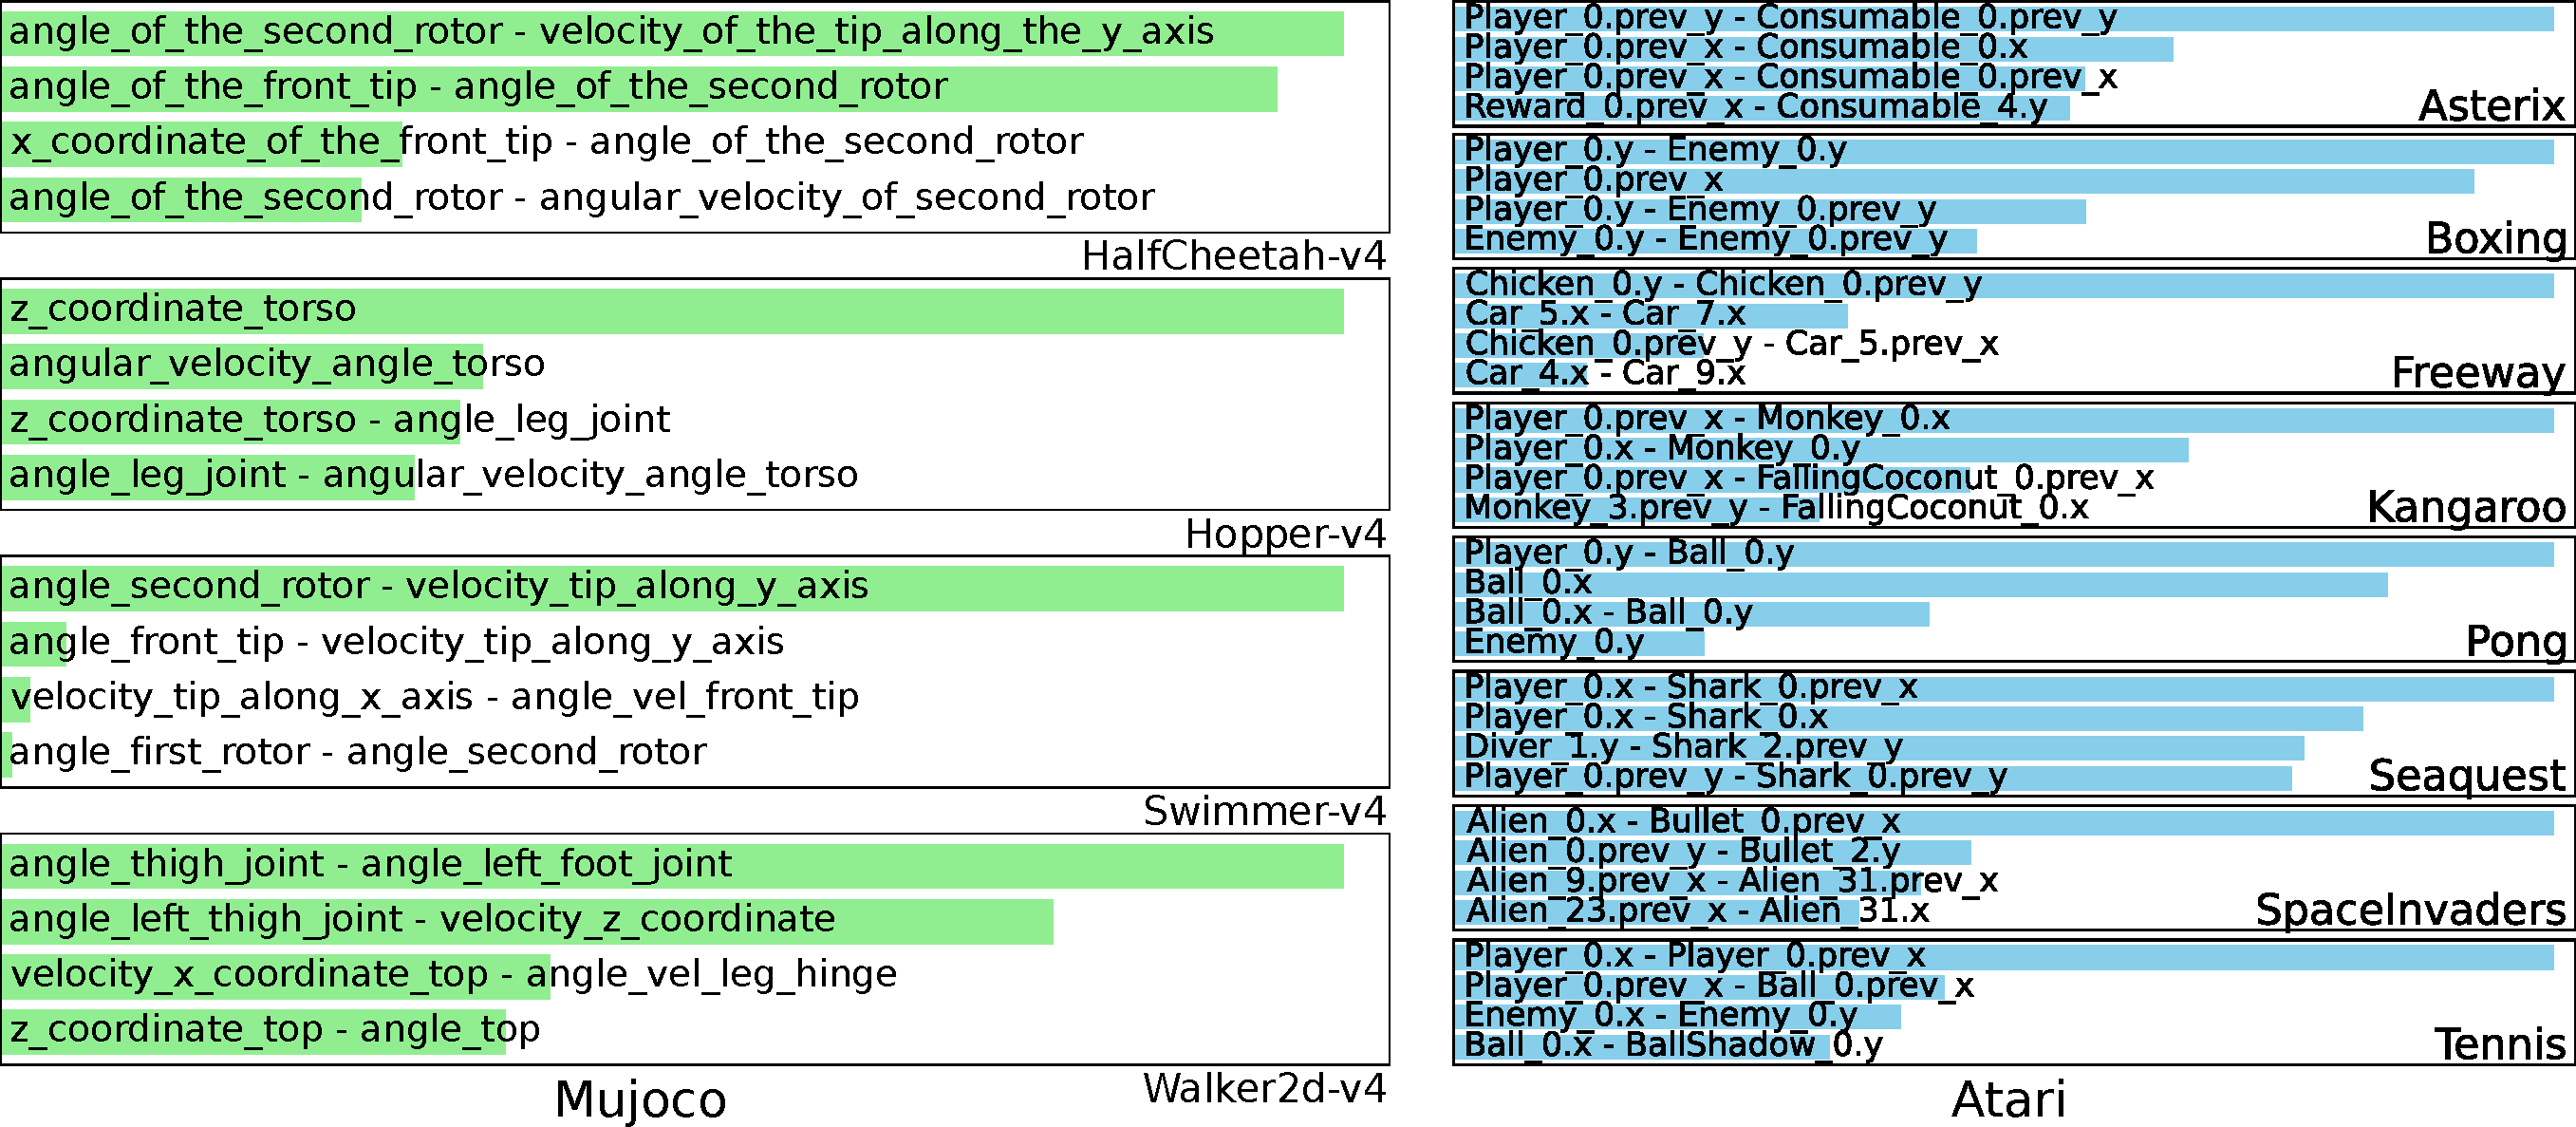
\includegraphics[trim={0 0 21cm 0},clip,width=0.7\textwidth]{images/images_part3/dis_mujoco+f_atari.pdf}
%   \caption{State features importance for MuJoCo environments given by medium-sized oblique decision trees.}\label{fig:mujoco-feat}
% \end{figure}
To validate the methodology proposed in the previous chapter, we imitated pre-trained experts neural network policies with various less complex policies.
We obtain diverse baselines policies with diverse interpretability measures and performances for a wide range of environments.
For each environment, we save the best baseline policy of each class in terms of RL objective (\ref{def:mdp-obj}) after unfolding.
We open source those best in class policies here:~\url{https://github.com/KohlerHECTOR/interpretable-rl-zoo}.
We hope that those transparent policies can help teaching and research in (interpretable) sequential decision making.
In the next chapter, we focus on those best in class unfolded policies and study how they trade off our metrics of interpretability and the RL objective~\ref{def:mdp-obj}.
